%%%%%%%%%%%%%%%%%%%%%%%%%%%%%%%%%%%%%%%%
%\vspace{0.1in}
\section{Related work}
\label{related}
%%%%%%%%%%%%%%%%%%%%%%%%%%%%%%%%%%%%%%%%

\subsection{Service Discovery}

There has been much work on service discovery in field of distributed systems. Etcd ~\cite{etcd} is a distributed key-value store based on directories and consensus. It uses RAFT ~\cite{raft} protocol, primaraly for multiple nodes to maintain identical logs of state changing commands. Any node in a raft cluster may be treated as the master. It will coordinate with the others to agree on which order state changes should happen in. Another work is Consul ~\cite{Consul} which is open source solution for service discovery and distributed configuration management. It has a distributed key, value store for storing service database that can be queried using DNS. Consul provides dynamic load balancing and comprehensive service health checking using both in-built solutions as well as user provided custom solutions. Unlike Consul, Synapse ~\cite{Synapse} was designed to support services running in Docker. At the core of Synapse is an HAProxy instance for routing requests from a service consumer on the application server to a service provider running in the cluster. HAProxy configuration in Synapse are made by “watchers” daemons that check for changes to the locations of services. Dynamic Service Discovery System with the help of Zookeeper ~\cite{zookeeper}, which provides an open source solution to the various coordination problems in large distributed systems.  ZooKeeper, as a centralized coordination service, is distributed and highly reliable, running on a cluster of servers called a ZooKeeper ensemble. Distributed consensus, group management, presence protocols, and leader election are implemented by the Zookeeper ensemble. 

The docker platform has Docker Swarm ~\cite{swarm} and Docker Compose ~\cite{compose} that, when combined together, may provide a solution to the service discovery problem. Swarm manager nodes assign each service in the swarm a unique DNS name and load balances running containers. One can query every container running in the swarm through a DNS server embedded in the swarm. Mesos-DNS ~\cite{mesos} provides service discovery through DNS. Mesos-DNS generates an service record for each application instances and translates these records to the IP address and port on the machine currently running each application.

It is important to distinguish the service discovery problem from “orchestration” - the process of deploying containers on a cluster of machines. CoreOS, Mesos/Mesosphere, OpenShift, CloudFoundry, Kubernetes, Brooklyn/Clocker, Shipyard, and Crane are just a few of the many available orchestration solutions, and some of the larger projects like Kubernetes and Mesosphere include some service discovery features. In general, orchestration solutions represent a fundamentally different approach to managing systems built with containers. Adoption of these solutions is often a very heavy undertaking requiring highly specialized deployment environments.

\subsection{Named Routing}

\begin{figure}
\centering
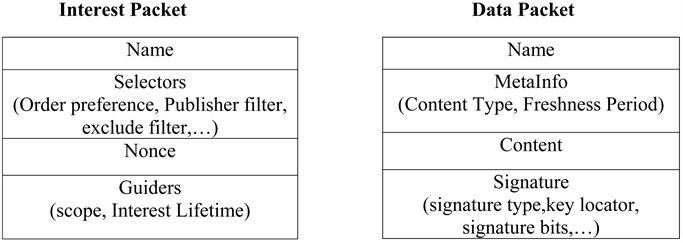
\includegraphics[height=3cm, width=8cm]{figs/ndn_packet.png}
\caption{\label{fig:ndn}NDN packets~\cite{ndn}}
\end{figure}
Information-Centric Networking (ICN) has been proposed as a promising new Internet architecture. In ICN, the content is accessed by the name of the content rather than the IP address of the host machine that has the content. By separating content from location, ICN is expected to improve the network efficiency and reduce the communication cost for fetching contents.  Similarly, Named data networking (NDN) ~\cite{ndn} is a new networking paradigm using named data instead of named hosts for communication under the broad ICN umbrella. NDN architecture makes the original Internet design elegant and powerful. NDN is driven by the receiving end through the exchange of two types of packets:
Interest and Data. Both types of packets carry a name that identifies a piece of data that can be transmitted in one Data packet. A consumer puts the name of a desired piece of data into an Interest packet and sends it to the network. Routers use this name to forward the Interest toward the data producer(s). Once the Interest reaches a node that has the requested data, the node will return a Data packet that contains both the name and the content, together with a signature by the producer’s key which binds the two (Fig 1). This Data packet follows in reverse the path taken by the Interest to get back to the requesting consumer. 

\begin{figure}
\centering
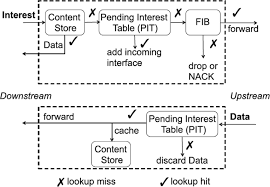
\includegraphics[height=3cm, width=8cm]{figs/process2.png}
\caption{\label{fig:process2}Forwarding Process at an NDN Node~\cite{ndn}}
\end{figure}

To carry out the Interest and Data packet forwarding functions, each NDN router maintains three data structures: a Pending Interest Table (PIT), a Forwarding Information Base (FIB), and a Content Store (CS) (Fig 2), as well as a Forwarding Strategy module that determines whether, when and where to forward each Interest packet. The PIT stores all the Interests that a router has forwarded but not satisfied yet. The Content Store is a temporary cache of Data packets the router has received. The forwarding information base (FIB) table use the names to route a request to next  hop routers that are closer to the data provider by performing longest-prefix matching. The hierarchy also allows name resolution and data routing information to be gathered across similar data source names, which is the key point to enhance scalability and flexibility of the network architecture. 




